\documentclass[12pt,a4j,final]{jreport}
\synctex=1
\usepackage{amsmath,amssymb,amsthm}
\usepackage{ascmac,amscd}
\usepackage{enumerate}
\usepackage{comment}
\usepackage{fancybox,fancyhdr}
%\usepackage[dvipdfmx]{hyperref}
\usepackage[dvipdfmx]{graphicx}
%\usepackage{pxjahyper}
\usepackage[margin=25mm]{geometry} %%% マージンは固定
\usepackage{here}
\usepackage{multicol}
\usepackage{mathtools} %行列の転置で使用
\usepackage[dvipdfmx]{graphicx}
\renewcommand{\bibname}{参考文献}


\theoremstyle{definition}
\newtheorem{Thm}{定理}[section]
\newtheorem{Pro}[Thm]{命題}
\newtheorem{Lem}[Thm]{補題}
\newtheorem{Cor}[Thm]{系}
\newtheorem{Def}[Thm]{定義}
\newtheorem{Ex}[Thm]{例}
\newtheorem{Not}[Thm]{記号}
\newtheorem{Rem}[Thm]{注意}
\newtheorem{Conj}[Thm]{予想}
\newtheorem*{Abs}{概要}
\newtheorem{Fact}{事実}[section]

\renewcommand{\proofname}{証明} 
 
\title{2025年度 卒業論文\\
\vspace{4\baselineskip}
超曲面論における積分公式
\vspace{4\baselineskip}
}
\author{
荒木 颯斗\\
飯田 祐貴\\
実松 直哉\\
多々良 勇太\\
三森 誠真\\
山本 裕也\\\\\\
東京理科大学\\
創域理工学部 数理科学科\\
馬場蔵人研究室
}
%\email{} %%% 入力不要
\date{} %%% 入力不要
\pagestyle{empty} %%% ページ番号はつけない


\begin{document}

\maketitle

\tableofcontents

\chapter{はじめに・卒論作成要領}

最終版ではこの章は削除します．

\section{作成前の注意事項}

\subsection{文章作成にあたって}

\begin{enumerate}[(1)]
\item 表紙のタイトルは教科書\cite{Koike}をもとに事前に作成しました．他に良いタイトルが思いつけば検討しましょう．
\item chapterのタイトルは教科書\cite{Koike}をもとに事前に作成しました．こちらも代案があればお願いします．
\item 各自の割り振りは括弧書きの部分にあたります．教科書で割り振りに合わせて分担してあります．
\item sectionに「タイトル」の部分は各自で適切なフレーズに変更してください．
ただし，（苗字）は文責を明確にするため消さずに残しておいてください．
\item 内容は教科書\cite{Koike}の完コピは内容として冗長になる場合があります．
数学的に重要であると思う内容をどうまとめていくかの作業に注力してください．
証明や計算も冗長になってないか検討してください．
\item 内容をまとめる際に，今回の執筆範囲にある定理・命題・補題等の番号は
この卒業論文ように改めて番号を付け直します．後述の$\backslash$labelコマンドを確認してください．
\item 一方，今回の執筆範囲からもれた定理・命題・補題を利用するときは，必ず本文中にその内容を述べてください．
\item 執筆にあたって数学の記号は教科書\cite{Koike}に従ってください．後述のフォントも確認すること．
\cite{Koike}で用意されていない記号の導入は自由に行って問題ありません．
\item 句読点は教科書\cite{Koike}に合わせて「．，」にすること．
\item フォントは本文は明朝体，タイトルはゴシック体が基本です．
\item 論文では「です・ます」調は避けてください．
\item 数学の論文は普遍的な事実を記述するものなので，
主語が「私」となる文はありません．
（謝辞などの例外はあります．その場合は「私」ではなく「著者」となります．）
\item 基本的な\TeX の使い方は\cite{OK}に従ってください．
（texファイルを一からすべてを作るのは大変なので，このサンプルファイルのtexファイルをもとにするのが効率的と思います．今回はフォーマットが決まっているのでAIはうまく働いてくれないかもしれません．）
\end{enumerate}


\section{生成系AIの利用にあたっての注意}

生成系AIの進歩に伴い論文執筆でも
利用される場面が出てきましたが，
その利用にあたっていくつか注意することがあります．

\begin{itemize}
\item 一般的に，論文に係る最終的な責任の所在は執筆者にあります．
生成系AIであることを免責理由とした主張は通りません．
\item いかなる理由があっても，
次のような情報を生成系AIに入力してはいけません．
\begin{enumerate}
\item[(1)]個人情報やプライバシー情報等の人格的利益を害する蓋然性のある情報
\item[(2)] 他者の名誉等の人格的利益を害することを目的とする虚偽の情報
\item[(3)] 他者の知的財産権や研究上の秘密等として扱うべき情報
\end{enumerate}
\item 生成系AI著作権侵害や研究倫理違反にあたる剽窃となる可能性を伴いますので，利用にあたっては特段の注意が必要になります．
\item 現時点での生成系AIに備わっている数学のレベルは高度な知識と厳格な論理展開を必要とする大学数学のレベルまで達しておらず，一見もっともらしい数学の文章を生成してくれます．
しかし，専門的な見地から見れば嘘の情報や矛盾した論理が露見されることがあります（ハルシネーション現象）．
\end{itemize}


\section{サンプル（オイラーの公式）}

本論のメインの章で用いる基本的な概念を用意しておくと構成がまとめやすいです．
大学1,2年までの内容は認めて，
本論の内容に書かれた内容を理解するために必要な数学的な概念を説明してください．
他にも
卒業研究のテキストを読むにあたって
必要な数学的な知識もここで準備しておくことで本論が整理されます．

\subsection{数の集合}

数の理論を卒業研究の内容に選ばない限りに，
ここまでさかのぼって概念を用意していく必要はありません．

\begin{Def}[サンプル]\label{Def:sample}
定理・命題・補題・系・定義・注意などには通し番号を振ってください．
（TeXでの作成を勧めている理由の一つ）
\end{Def}


\begin{screen}
\begin{itemize}
\item 定理環境の雛形・$\backslash$labelコマンドの使い方\\
\verb|\begin{Thm}[option]\label{labelname}|\\
...\\
\verb|\end{Thm}|\\
\item \verb|[option]|は見出しを付けたいときに便利ですが，不要な場合は削除してください．定義\ref{Def:sample}では
\verb|[サンプル]|が入力されたときの出力になっています．
\item \verb|\begin{Thm} ... \end{Thm}|の「\verb|Thm|」の部分を
\verb|Def|, \verb|Pro|, \verb|Lem|, \verb|Cor|
に置き換えると，定義，命題，補題，系になるように設定してあることが
ソースの17行目付近を見れば確認できます．
\item この定理を引用するときは\verb|\label{labelname}|を事前に入力しておきます．
\item 引用するときのコマンドは\verb|\ref{labelname}|です．
\item[] 入力例：定理\verb|\ref{labelname}| から ...
\item 他の方が引用をできるためのルールです．labelnameは教科書の定理等をlabel付けるときは次のような雛形に従ってください．
\item 教科書\cite{Koike}のp.~148, 定理2.9.2の内容を記載する場合：
\begin{screen}
\verb|\begin{Thm}\label{Koike2.9.2}|\\
...\\
\verb|\end{Thm}|\\

\end{screen}
\end{itemize}
\end{screen}

\begin{proof}
.........
右の通りハルモスの四角形は自動で挿入されます．
\end{proof}

\begin{screen}
\begin{itemize}
\item 証明環境の雛形\\
\verb|\begin{proof}|\\
...\\
\verb|\end{proof}|
\item 必要に応じて31行目\verb|\renewcommand{\proofname}{証明}|を編集すること．
\item また，一時的に「証明」の出力を変更したいときは次のような方法もある\\
\verb|\begin{proof}[証明（スケッチ）]|\\
...\\
\verb|\end{proof}|
\end{itemize}
\end{screen}

\begin{Rem}
数式は \$y=f(x)\$ のように\$で囲むのがルールです．
本来では$y=f(x)$と表示されるものが，
\$\$で囲まないと y=f(x) がそのまま表示されて修正の対象です．
場合によっては適切にコンパイルが通らないことが起こります．

また，TeXでやってはいけないことの一つに，
半角で入力した数式以外のものを\$\$で囲んではいけません．
\begin{itemize}
\item ダメ：「\$サンプル\$」
\item 例外処理：「\$$\backslash \verb|text|\{\text{サンプル}\}$\$」
\end{itemize}
\end{Rem}


\subsection{実数の絶対値}

場合分けを書き方は次を参考にすること：

\begin{equation}
|a|=\begin{cases}
a  & (a \geq 0) \\
-a & (a < 0)
\end{cases}
\end{equation}

\section{表・図の挿入例}

表や図を挿入してわかりやすい表現を心掛けることを推奨しています．
表や図の挿入方法は次を参考にしてください．

\begin{table}[H]
\centering
\caption{数の集合（表には見出しを付けてください．位置は表の上です．著作権が著者でなければ，その所在を明記してください．）}

\scalebox{0.8}{
\begin{tabular}{|c|c|}
\hline
記号 & 意味\\
\hline
\hline
$\mathbb{O}$ & 八元数全体 \\
$\mathbb{H}$ & 四元数全体 \\
$\mathbb{C}$ & 複素数全体\\
$\mathbb{R}$ & 実数全体\\
$\mathbb{Q}$ & 有理数全体\\
$\mathbb{Z}$ & 整数全体\\
$\mathbb{N}$ & 自然数全体\\
\hline
\end{tabular}
}
\end{table}


\begin{figure}[H]
\centering

\includegraphics[width=5cm]{symbole03.jpg}
\caption{理科大シンボル
\cite{tus}
（図の見出しも必須です．位置は図の下です．著作権が著者でなければ，その所在を明記してください．）}
\end{figure}


\dotfill

\dotfill

\dotfill

\dotfill

\dotfill （文章が続く）

\begin{Thm}[オイラーの公式]\label{thm:Euler}
任意の$\theta\in \mathbb{R}$に対して，
\begin{equation}\label{eqn:Euler}
e^{i\theta}=\cos\theta+i\sin\theta.
\end{equation}
\end{Thm}

\begin{Cor}[博士の愛した数式]
\begin{equation*}
e^{i\pi}=-1.
\end{equation*}
\end{Cor}


\begin{proof}[証明]
(\ref{eqn:Euler})式において，$\theta=\pi$を代入せよ．
\end{proof}


\subsection{主定理の証明のための準備}

\noindent
定理\ref{thm:Euler}を証明するために
次の命題を用意する．

\begin{Pro}[$e^{x}$のマクローリン展開]
\begin{equation}\label{pro:exp}
e^{x}=\sum_{n=1}^{\infty}\dfrac{1}{n!}x^{n}
\quad
(\forall x\in\mathbb{R}).
\end{equation}
\end{Pro}

\begin{proof}[証明]
直接計算によって$e^{x}(=:f(x))$の$n$階導関数は$e^{x}$である．
また，$a_{n}=f^{(n)}(0)/n!=1/n!$とすると，
\begin{equation*}
\dfrac{a_{n+1}}{a_{n}}=\dfrac{1}{n+1} \to 0
\quad(n \to \infty).
\end{equation*}
よって，ダランベールの収束判定法より(\ref{pro:exp})が従う．
\end{proof}

\begin{itembox}[l]{証明を書くにあたって} % c=center, l=left, r=right
\begin{itemize}
\item 証明は要点をおさえていればOKです．
\item 証明中に煩雑な計算が続くときは付録にまわすことも1つのやり方です．
\item 証明環境の利用を忘れずに．
\end{itemize}
\end{itembox}


\begin{Lem}[$\cos x, \sin x$のマクローリン展開]
任意の$x\in \mathbb{R}$に対して，
\begin{align*}
\cos x &= \sum_{n=0}^{\infty}\dfrac{(-1)^{n}}{(2n)!}x^{2n},\\
\sin x &= \sum_{n=0}^{\infty}\dfrac{(-1)^{n}}{(2n+1)!}x^{2n+1}.\\
\end{align*}
\end{Lem}

\begin{proof}[証明]
命題\ref{pro:exp}と同様な議論で示される．
\end{proof}


\subsection{主定理の証明}

\begin{proof}[定理$\ref{thm:Euler}$の証明]
指数関数$e^{x}$および三角関数$\cos x, \sin x$の
定義域$x$は複素平面全体に正則関数として拡張できることから，
\begin{align*}
e^{i\theta}
&= \sum_{n=0}^{\infty}\dfrac{1}{n!}(i\theta)^{n}\\
&= \sum_{n=0}^{\infty}\dfrac{i^{2n}}{(2n)!}\theta^{2n}
+ \sum_{n=0}^{\infty}\dfrac{i^{2n+1}}{(2n+1)!}\theta^{2n+1}\\
&= \sum_{n=0}^{\infty}\dfrac{(-1)^{n}}{(2n)!}\theta^{2n}
+ i\sum_{n=0}^{\infty}\dfrac{(-1)^{n}}{(2n+1)!}\theta^{2n+1}\\
&= \cos\theta + i\sin\theta.
\end{align*}
したがって，主張を得る．
\end{proof}

長い式変形が続くときは\verb|align|環境を利用すると，
改行後の等号の位置を揃えることができます．

\section*{代表的な数式フォント}

分野ごとに標準的に使われる数式フォントが列挙しました．

\begin{itemize}
\item 入力：\verb|$ABCDEFGHIJKLMNOPQRSTUVWXYZ$|
\item 出力：$ABCDEFGHIJKLMNOPQRSTUVWXYZ$
\item[]
\item 入力：\verb|$abcdefgehijlmnopqrstuvwxyz$| 
\item 出力：$abcdefgehijlmnopqrstuvwxyz$
\item[]
\item 入力：\verb|$\mathcal{ABCDEFGHIJKLMNOPQRSTUVWXYZ}$|
\item 出力：$\mathcal{ABCDEFGHIJKLMNOPQRSTUVWXYZ}$
\item[]
\item 入力：\verb|$ABCDEFGHIJKLMNOPQRSTUVWXYZ$| 
\item 出力：$\mathfrak{ABCDEFGHIJKLMNOPQRSTUVWXYZ}$
\item[]
\item 入力：\verb|$abcdefgehijlmnopqrstuvwxyz$|
\item 出力：$\mathfrak{abcdefgehijlmnopqrstuvwxyz}$
\end{itemize}





\chapter{超曲面（三森・山本・荒木）}

\section{正則局所超曲面の定義（三森）}
%%% ここから入力 %%%
この節において, \ $C^r$級, \ さらに一般に, \ 区分的に$C^r$級の超曲面の概念を定義する.
最初に, \ $C^r$超曲面の構成要素である$C^r$正則局所超曲面の概念を定義する.
以下, \ $n \geq 2$ とする.
領域 $D \subset \mathbb{R}^{n}$ とし, \ $C^{r}$ 写像 $\boldsymbol{x}: D \rightarrow \mathbb{E}^{n+1}$ を考える.
つまり, \ $\vec{\boldsymbol{x}}\left(u_{1}, \cdots, u_{n}\right)=\overrightarrow{o\boldsymbol{x}\left(u_{1}, \cdots, u_{n}\right)} \quad\left(\left(u_{1}, \cdots, u_{n}\right) \in D\right)$ によって定義される.
ベクトル値関数 $\vec{\boldsymbol{x}}: D \rightarrow \mathbb{R}^{n+1}$ が $C^{r}$ 級であるとする.
$\vec{\boldsymbol{x}}\left(u_{1}, \cdots, u_{n}\right)=\left(x_{1}\left(u_{1}, \cdots, u_{n}\right), \cdots, x_{n+1}\left(u_{1}, \cdots, u_{n}\right)\right) \quad$ として, \ $D$上の行列値関数
$J \boldsymbol{x}=　\prescript{t\!}{}{\left(\begin{array}{ccc}
\frac{\partial x_{1}}{\partial u_{1}} & \cdots & \frac{\partial x_{n+1}}{\partial u_{1}} \\ 
\vdots & \ddots & \vdots \\ 
\frac{\partial x_{1}}{\partial u_{n}} & \cdots & \frac{\partial x_{n+1}}{\partial u_{n}}\end{array}\right)}$ 
は$\boldsymbol{x}$ の$\textbf{ヤコビ行列}$とよばれる.
$D$の各点において, \ $\operatorname{rank} J \boldsymbol{x} = n$ であるとき,
$\boldsymbol{x}: D \rightarrow \mathbb{E}^{n+1}$ を $\mathbb{E}^{n+1}$ 内の $\boldsymbol{C^{r}} \textbf{正則局所超曲面}$（$C^{r}$ はめ込み）といい, 
その像 $S:= \boldsymbol{x}(D)$ を $\boldsymbol{C^r} \textbf{超曲面片}$ という.

\begin{Pro}\label{Koike1.9.1}
 $\boldsymbol{x}: D \rightarrow \mathbb{E}^{n+1}$ が $C^{r}$ 正則局所超曲面であるとき, \ $\dfrac{\partial \vec{\boldsymbol{x}}}{\partial u_{1}}, \cdots$ ，$\dfrac{\partial \vec{\boldsymbol{x}}}{\partial u_{n}}$ は $1$ 次独立である（図\ref{figure1.9.1}を参照）.
\end{Pro}

\begin{figure}[h]
  \centering
  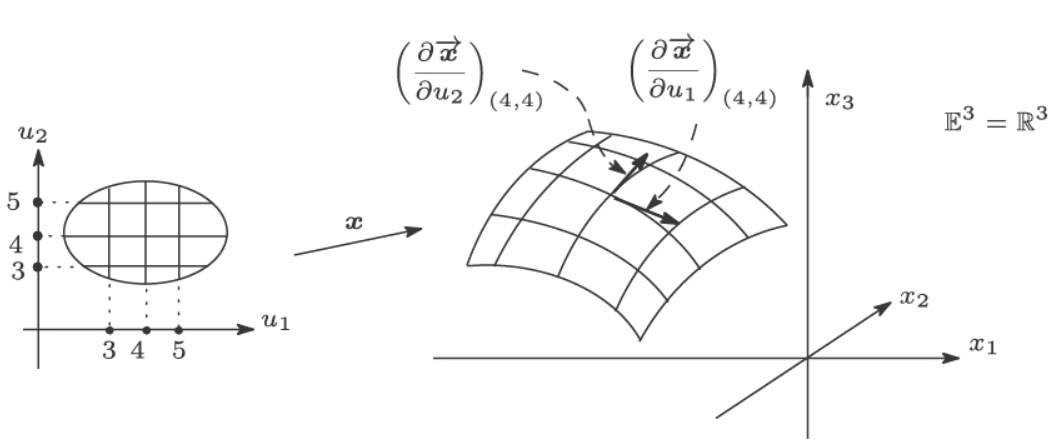
\includegraphics[width=15cm]{figure1.9.1.png}
  \caption{$\mathbb{E}^3$内の$C^r$正則局所超曲面[2]}
  \label{figure1.9.1}
\end{figure}

\begin{proof}[\textbf{証明の概略}]
$\boldsymbol{x}$ は$C^r$正則局所超曲面なので, \ $D$の各点でrank $J \boldsymbol{x} = n$ であり, \ ${}^t J \boldsymbol{x}$ の第 $1$ 行, $\cdots$ , 第 $n$ 行の定める行ベクトルは各々, \ $\dfrac{\partial \vec{\boldsymbol{x}}}{\partial u_{1}}, \ldots ., \dfrac{\partial \vec{\boldsymbol{x}}}{\partial u_{n}}$ であるので, \ $1$次独立である.（行列のランクと$1$ 次独立な行ベクトルの最大個数が一致することより）
\end{proof}

\bigskip

以下, \ $C^r$ 正則局所超曲面 $\boldsymbol{x}: D \rightarrow \mathbb{E}^{n}$ はすべて単射であるとする.
$C^{r}$ 正則局所超曲面 $\boldsymbol{x}= \boldsymbol{x} \left(u_{1}, \cdots, u_{n}\right) \quad ((u_{1}, \cdots, u_{n}) \in D )$ に対し,
$\boldsymbol{x}^{-1}=\left(u_{1}, \cdots, u_{n}\right): S:=\boldsymbol{x}(D) \rightarrow \mathbb{R}^{n}$ を $C^{r}$ 超曲面片 $S$ の\textbf{座標}という.
各 $i \in\{1, \cdots, n\}$ に対し, \ $S(= \boldsymbol{x}(D))$ 上の曲線 $u_{i} \mapsto \boldsymbol{x}\left(a_{1}, \ldots, a_{i-1}, u_{i}, a_{i+1}, \cdots, a_{n}\right)$
($a_{1}, \cdots, a_{n}$ : 定数 ) を $\boldsymbol{u_{i}}$ \textbf{曲線}とよび, \ これらをまとめて $S$ の\textbf{座標曲線}とよぶ.
点$p = \boldsymbol{x} (a_{1}, \cdots, a_{n}) \in S$ に対し, 
$\left(\dfrac{\partial}{\partial u_{i}}\right)_{p}:=\left(\dfrac{\partial \vec{\boldsymbol{x}}}{\partial u_{i}}\right)_{\left(a_1, \cdots, a_{n}\right)}(i=1, \cdots, n)$ とおく.
$\left(\dfrac{\partial}{\partial u_{1}}\right)_{p}, \cdots,\left(\dfrac{\partial}{\partial u_{n}}\right)_{p}$ によって生成される数ベクトル空間$\mathbb{R}^{n+1}$ の$n$ 次元部分ベクトル空間を$S$ の $p$ における\textbf{接空間}といい, \ $T_p S$ で表す. また, \ $T_p S$ の各元を$S$ の $p$ における\textbf{接ベクトル}という.
各点 $p$ に対し, \ $\left(\dfrac{\partial}{\partial u_{i}}\right)_{p}$ を対応させる対応 $\dfrac{\partial}{\partial u_{i}}(i=1 , \cdots, n)$ の順序対 $\left(\dfrac{\partial}{\partial u_{1}}, \ldots, \dfrac{\partial}{\partial u_{n}}\right)$ を $S$ の\textbf{座標基底場（自然基底場）}という.\\
また, \ $T_p S$ の直交補空間 $\left(T_{p} S\right)^{\perp}:=\left\{\boldsymbol{u} \in \mathbb{R}^{n+1} \mid \forall \boldsymbol{w} \in T_{p} S, \boldsymbol{u} \cdot \boldsymbol{w} =0\right\}$ を $S$ の $p$ における\textbf{法空間}という. また, \ $T_{p}^{\perp} S$ の各元を $S$ の $p$ における\textbf{法ベクトル}という.
$\quad \operatorname{dim} T_{p}^{\perp} S=\operatorname{dim} \mathbb{R}^{n+1}-\operatorname{dim} T_{p} S=(n+1)-n=1$ であることに注意しておく.

\bigskip

\begin{Pro}\label{Koike1.9.2}
  $\boldsymbol{x}: D \rightarrow \mathbb{E}^{n+1}$ を $C^{r}$ 正則局所超曲面とし, \ $\varphi$ を$\mathbb{R}^n$のある $D^{\prime}$ から$D$ への$C^r$同型写像とする. このとき, \ $\boldsymbol{x} \circ \varphi: D^{\prime} \rightarrow \mathbb{E}^{n+1}$も $C^{r}$ 正則局所超曲面になる.
\end{Pro}


\begin{proof}
  $\boldsymbol{x}^{-1}=\left(u_{1}, \cdots, u_{n}\right), \ (\boldsymbol{x} \circ \varphi)^{-1}=\left(\bar{u}_{1}, \cdots, \bar{u}_{n}\right)$ とする. このとき, \ 合成関数の連鎖律により, \ 
\begin{equation}\label{eq1.9.1}
  \dfrac{\partial(\overrightarrow{\boldsymbol{x} \circ \varphi})}{\partial \bar{u}_{i}}
=\displaystyle \sum_{j=1}^{n} \dfrac{\partial \vec{\boldsymbol{x}}}{\partial u_{j}} \cdot \dfrac{\partial u_{j}}{\partial \bar{u}_{i}}
\end{equation}
 が成り立つ.
この式から, \ 
\begin{equation}
  J(\boldsymbol{x} \circ \varphi)
  =J \boldsymbol{x} \cdot J \varphi
=J \boldsymbol{x} \left(\begin{array}{ccc}\frac{\partial u_{1}}{\partial \bar{u}_{1}} & \cdots & \frac{\partial u_{1}}{\partial \bar{u}_{n}} \\ \vdots & \ddots & \vdots \\ \frac{\partial u_{n}}{\partial \bar{u}_{1}} & \cdots & \frac{\partial u_{n}}{\partial \bar{u}_{n}}\end{array}\right).
\end{equation}
右辺における行列は$\varphi$ のヤコビ行列であり, \ $\varphi$ が$C^r$同型写像であることから, \ $J \varphi$ は正則行列である.
したがって, \ 各点において $\operatorname{rank} J(\boldsymbol{x} \circ \varphi)=n$ であることがわかり, \ $\boldsymbol{x} \circ \varphi$ が $C^{\infty}$ 正則局所超曲面 であることが示される.
\end{proof}




\section{タイトル（山本）}
%%% ここから入力 %%%



\section{タイトル（荒木）}
%%% ここから入力 %%%




\chapter{超曲面論における変分公式（山本・荒木・飯田・実松）}\label{chap:conclusion}

\section{タイトル（山本）}
%%% ここから入力 %%%



\section{タイトル（荒木）}
%%% ここから入力 %%%



\section{タイトル（飯田）}
%%% ここから入力 %%%





\section{タイトル（実松）}
%%% ここから入力 %%%





\chapter{超曲面論におけるストークスの定理（多々良・三森）}


\section{タイトル（多々良）}
%%% ここから入力 %%%



\section{曲面上の$1$次微分形式に対するストークスの定理（三森）}

$C^{\infty}$ 曲面上の$C^r$ 級の$1$次微分形式に対し, \ 次のストークスの定理が成り立つ.

\begin{Thm}\label{Koike2.7.1}
  $\omega$ を $C^{\infty}$ 曲面 $(S, \mathcal{D})$ 上の $C^{r}$ 級 $1$ 次微分形式とし, \ 
$S^{\prime}$を区分的に $C^{r}$ 級の境界をもつ$S$の有界閉領域とする.
$c:[a, b] \rightarrow S$ を $S^{\prime}$ の境界 $\partial S^{\prime}$ を与える $S$ 上の区分的に $C^r$ 級の単純閉曲線
で, \ $S_{\lambda} \cap c([a, b]) \neq \phi$ となるような各$\lambda \in \Lambda$に対し, \
$\boldsymbol{x}_{\lambda}^{-1}=\left(u_{1}, u_{2}\right)$ として, \  $\left(d u_{1} \wedge d u_{2}\right)_{c(t)} \left(\overline{\boldsymbol{N}}_{c(t)}, \vec{c'}(t)\right)>0$
ようなものとする.
ここで$\overline{\boldsymbol{N}}$ は, \ $c([a, b])$ の$S$における単位法ベクトル場で$S'$からみて外側向きのものを表す. このとき, \ 次式が成り立つ.

$$
\displaystyle \int_{S'} d\omega = \int_c \omega.
$$

\end{Thm}

\begin{proof}
 $S'$がある $S_{\lambda}$ に含まれる場合を考える.
$\boldsymbol{x}_{\lambda}^{-1}=\left(u_{1}, u_{2}\right)$ とし, \ $E:=\boldsymbol{x}_{\lambda}^{-1}\left(S^{\prime}\right)$ とおく.
$S^{\prime}$ をいくつかの $[0,1] \times[0,1]$ を定義域とする区分的に $C^r$級の境界をもつ $C^{\infty}$ 超曲面片 $S_{\alpha}^{\prime}=\hat{\boldsymbol{x}}_{\alpha}([0,1] \times[0,1])(\alpha = 1, \cdots, l)$ たちに分割する.
ただし, \ $\hat{\boldsymbol{x}}_{\alpha}$ は $J\left(\boldsymbol{x}_{\lambda}^{-1} \circ \hat{\boldsymbol{x}}_{\alpha}\right)>0$ となるようにとる.
$C^{r}$ 曲線 $c_{j}^{\alpha}:[0,1] \rightarrow \mathbb{E}^{3}(j=1, \cdots, 4)$ を, \ 

$$
\begin{array}{lll}
c_{1}^{\alpha}\left(u_{1}\right):=\hat{\boldsymbol{x}}_{\alpha}\left(u_{1}, 0\right), & c_{3}^{\alpha}\left(u_{1}\right):=\hat{\boldsymbol{x}}_{\alpha}\left(1-u_{1}, 1\right) & \left(0 \leqq u_{1} \leqq 1\right) \\
c_{2}^{\alpha}\left(u_{2}\right):=\hat{\boldsymbol{x}}_{\alpha}\left(1, u_{2}\right), & c_{4}^{\alpha}\left(u_{2}\right):=\hat{\boldsymbol{x}}_{\alpha}\left(0,1-u_{2}\right) & \left(0 \leqq u_{2} \leqq 1\right)
\end{array}
$$
\noindent
によって定義する.
$c_{1}^\alpha \sim c_{4}^\alpha$ 
を順に結んでできる区分的に滑らかな閉曲線を
$c_\alpha$ と表す.
(このとき, \ 明らかに$c_\alpha$ は $\partial S_{\alpha}^{\prime}$ を与える単純閉曲線で
$\boldsymbol{x}_{\lambda}^{-1} \circ c_{\alpha}$ が反時計回りに進むようなものである.）
最初に, \ 各 $\alpha \in \{1, \cdots, l\}$ に対し, \  
$\displaystyle \int_{S_{\alpha}^{\prime}} d \omega = 
\int_{c_{\alpha}} \omega$ が成り立つことを示す.
$\hat{\boldsymbol{x}}_{\alpha}^{-1} = 
\left(u_{1}^{\alpha}, u_{2}^{\alpha}\right)$ とし,
$\omega = 
\displaystyle \sum_{i=1}^{2} f_{i}^{\alpha} d u_{i}^{\alpha}$
とする．
このとき, \ $d \omega=\left(-\left(\frac{\partial\left(f_{1}^{\alpha} \circ \hat{\boldsymbol{x}}_{\alpha}\right)}{\partial u_{2}^{\alpha}} \circ \hat{\boldsymbol{x}}_{\alpha}^{-1}\right)
+
\left(\frac{\partial\left(f_{2}^{\alpha} \circ \hat{\boldsymbol{x}}_{\alpha}\right)}{\partial u_{1}^{\alpha}} \circ \hat{\boldsymbol{x}}_{\alpha}^{-1}\right)\right) d u_{1}^{\alpha} \wedge d u_{2}^{\alpha}$ となる.
それゆえ, 
$$
\begin{aligned}
\displaystyle \int_{S_{\alpha}^{\prime}} d \omega 
&= 
\int_{0}^{1} \int_{0}^{1}
\left(
\underbrace{
-\frac{\partial (f_{1}^{\alpha} \circ \hat{\boldsymbol{x}}_{\alpha} )}{\partial u_{2}^{\alpha}}
}_{I_1}
+
\underbrace{
\frac{\partial (f_{2}^{\alpha} \circ \hat{\boldsymbol{x}}_{\alpha} )}{\partial u_{1}^{\alpha}}
}_{I_2}
\right) 
d u_{1}^{\alpha} d u_{2}^{\alpha} \\
&=
-\int_{0}^{1}\left(\left(f_{1}^{\alpha} \circ \hat{\boldsymbol{x}}_{\alpha}\right)\left(u_{1}^{\alpha}, 1\right)-\left(f_{1}^{\alpha} \circ \hat{\boldsymbol{x}}_{\alpha}\right)\left(u_{1}^{\alpha}, 0\right)\right) d u_{1}^{\alpha} \quad 
( I_{1} \text{を} u_{2}^{\alpha} \text{で積分}) \\
& \ \ \ \ +
\int_{0}^{1}\left(\left(f_{2}^{\alpha} \circ \hat{\boldsymbol{x}}_{\alpha}\right)\left(1, u_{2}^{\alpha}\right)-\left(f_{2}^{\alpha} \circ \hat{\boldsymbol{x}}_{\alpha}\right)\left(0, u_{2}^{\alpha}\right)\right) d u_{2}^{\alpha} 
\quad ( I_{2} \text { を } u_{1}^{\alpha} \text { で積分 }) \\
&= 
\int_{0}^{1}\left(-\left(f_{1}^{\alpha} \circ \hat{\boldsymbol{x}}_{\alpha}\right)(t, 1)+\left(f_{1}^{\alpha} \circ \hat{\boldsymbol{x}}_{\alpha}\right)(t, 0)+\left(f_{2}^{\alpha} \circ \hat{\boldsymbol{x}}_{0}\right)(1, t)-\left(f_{2}^{\alpha} \circ \hat{\boldsymbol{x}}_{\alpha}\right)(0, t)\right) d t
\end{aligned}
$$
\noindent
が示される.

次に, \ $\displaystyle \int_{c_\alpha} \omega$ 側を計算していく.

$$
\begin{aligned}
\int_{c_{1}^{\alpha}} \omega + \int_{c_{3}^{\alpha}} \omega
&=
\int_{0}^{1} \omega_{c_{1}^{\alpha}(t)}((\overrightarrow{c_{1}^{\alpha}})^{\prime}(t)) d t
+
\int_{0}^{1} \omega_{c_{3}^{\alpha}(t)}(( \overrightarrow{c_{3}^{\alpha}})^{\prime}(t)) dt \\
& =
\int_{0}^{1}\left(f_{1}^{\alpha}\left(c_{1}^{\alpha}(t)\right) \frac{d u_{1}^{\alpha}\left(c_{1}^{\alpha}(t)\right)}{d t}
+
f_{2}^{\alpha}\left(c_{1}^{\alpha}(t)\right) \frac{d u_{2}^{\alpha}\left(c_{1}^{\alpha}(t)\right)}{d t}\right) dt \\
& \ \ \ \ +
\int_{0}^{1}\left(f_{1}^{\alpha}\left(c_{3}^{\alpha}(t)\right) \frac{d u_{1}^{\alpha}\left(c_{3}^{\alpha}(t)\right)}{d t}
+
f_{2}^{\alpha}\left(c_{3}^{\alpha}(t)\right) \frac{d u_{2}^{\alpha}\left(c_{3}^{\alpha}(t)\right)}{dt}\right) dt \\
& =\int_{0}^{1}\left(\left(f_{1} \circ \hat{\boldsymbol{x}}_{\alpha}\right)(t, 0)-\left(f_{1}{ }^{\alpha} \circ \hat{\boldsymbol{x}}_{\alpha}\right)(1-t, 1)\right) d t \\
& =\int_{0}^{1}\left(\left(f_{1}^{\alpha} \circ \hat{\boldsymbol{x}}_{\alpha}\right)(t, 0)-\left(f_{1}^{\alpha} \circ \hat{\boldsymbol{x}}_{\alpha}\right)(t, 1)\right) dt
\end{aligned}
$$
\noindent
また
$\displaystyle \int_{c_{2}^{\alpha}} \omega
+\int_{c_{4}^{\alpha}} \omega$ についても同様にして

\begin{equation*}
 \displaystyle \int_{c_{2}^{\alpha}} \omega + \int_{c_{4}^{\alpha}} \omega
= \int_{0}^{1}\left(\left(f_{2}^{\alpha} \circ \hat{\boldsymbol{x}}_{\alpha}\right)(1, t)-\left(f_{2}^{\alpha} \circ \hat{\boldsymbol{x}}_{\alpha}\right)(0, t)\right) d t 
\end{equation*}
が示される.

以上より, \ $\displaystyle \int_{S_{\alpha}^{\prime}} d \omega = \int_{c_{a}} \omega$.

したがって, \ $\displaystyle \int_{S^{\prime}} d \omega
=\sum_{\alpha=1}^{l} \int_{S_{\alpha}^{\prime}} d \omega
=\sum_{\alpha=1}^{l} \int_{c_{\alpha}} \omega 
=\int_{c} \omega$.

\end{proof}

これを踏まえたうえで, \ 区分的に $C^r$ 級の境界をもつ $C^r$ 超曲面片 $S = \boldsymbol{x}(E)$ 上での積分公式 $\displaystyle \int_{S} \operatorname{rot} \boldsymbol{X} \cdot d\boldsymbol{A}
=\int_{c} \boldsymbol{X} \cdot d \boldsymbol{r}$ が定理\ref{Koike2.7.1}の特別な場合であることを説明する.

$\boldsymbol{x}^{-1} = (u_{1}, u_{2})$ として, \ $S$ 上の $C^{r}$ 級の $1$ 次微分形式 $\omega$ を 
$\omega:= \displaystyle \sum_{i=1}^{2}(\boldsymbol{X} |_S) \cdot\left(\frac{\partial \boldsymbol{x}}{\partial u_{i}} \circ \boldsymbol{x}^{-1}\right) d u_{i} \quad$ によって定める.\\
このとき, \ $d \omega = 
\operatorname{rot} \boldsymbol{X} \cdot\left(\left(\frac{\partial \boldsymbol{x}}{\partial u_{1}} \times \frac{\partial \boldsymbol{x}}{\partial u_{2}}\right) \circ \boldsymbol{x}^{-1}\right) 
d u_{1} \wedge d u_{2} \quad$ となり,
\begin{equation*}
  \displaystyle \int_{S} \operatorname{rot} \boldsymbol{X} \cdot d \boldsymbol{A} =
\int_{S} d \omega
\end{equation*}
となることがわかる. 一方,\\
$\omega_{c(t)} (\overrightarrow{c^{\prime}}(t)) d t
=
\left(\boldsymbol{X}|_{S}\right)_{c(t)} \cdot \overrightarrow{c^{\prime}}(t) d t \quad$ となり,

$$
\int_{c} \boldsymbol{X} \cdot d \boldsymbol{r} = \int_{c} \omega
$$

\noindent
となることがわかる.

よって,
$\displaystyle \int_{S} \operatorname{rot} \boldsymbol{X} \cdot d \boldsymbol{A}
=\int_{c} \boldsymbol{X} d \boldsymbol{r}$ となり, \ 定理\ref{Koike2.7.1} の特別な場合であることがわかる.


\chapter{超曲面論におけるガウス・ボンネの定理（山本・荒木・飯田）}

\section{タイトル（山本）}
%%% ここから入力 %%%


\section{タイトル（荒木）}
%%% ここから入力 %%%


\section{タイトル（飯田）}
%%% ここから入力 %%%

\section{タイトル（実松）}
%%% ここから入力 %%%


\section{タイトル（多々良）}
%%% ここから入力 %%%









%%% 参考文献を記載してください

\begin{thebibliography}{99}
\thispagestyle{empty} %%% ページ番号はつけない
\bibitem{format} 著者, タイトル, 出版社, 発行年をこの順番で記載してください
\bibitem{Koike} 小池直之, 積分公式で啓くベクトル解析と微分幾何学, 共立出版, 2022年
\bibitem{OK} 奥村晴彦・黒木祐介, Latex 2$\varepsilon$美文書作成入門（第$7$版）,
技術評論社，2017年
\bibitem{tus} 東京理科大学公式ホームページ\verb|https://www.tus.ac.jp/|
\end{thebibliography}

\end{document}
